\section{\name{} Prototype}
\label{sec:prototype}
In order to evaluate the expected performance of a \name{}, we built a prototype in Chisel~\cite{chisel} and C on top of the open source RISC-V Rocket Core system~\cite{rocket-chip} and evaluated performance using cycle-accurate hardware simulations~\cite{verilator}.

Figure~\ref{fig:nanoPU-prototype} shows a high-level block diagram of the prototype's most relevant components.
The prototype implements the main components of the NIC described in \S\ref{sec:nanoPU} and connects it to a slightly modified RISC-V Rocket core.
The prototype implements the following aspects of the \name{}:
\begin{itemize}
    \item The NIC Datapath, without a hardware transport protocol, encryption/decryption or MAC processing.
    \item The NIC-Core Interface, including small changes to the core required to add the fast path into the register file.
    \item The NIC hardware thread scheduler and nanoKernel.
\end{itemize}
Since the NIC and core run at the same clock rate in our prototype, we have no need for clock domain crossing (CDC) FIFOs in the NIC-Core Interface. \steve{Check if we are still describing the CDC FIFOs in the NIC-Core Interface description}
Furthermore, since the prototype does not implement a transport protocol, we assume that all messages sent and received by the applications consist of a single Ethernet packet, which we believe will be true for the vast majority of nanoservice applications.

To provide a useful reference, we compare the performance of our \name{} prototype to a RISC-V Rocket Core with a traditional DMA-based NIC called IceNIC~\cite{firesim}.
Figure~\ref{fig:icenic-prototype} depicts a block diagram of the IceNIC RISC-V system.
IceNIC behaves in a similar fashion to Intel DDIO based NICs.
That is, it uses DMA to move network packets directly between the NIC and the CPU's last level cache.
Since the IceNIC RISC-V design is an integrated solution, it does not include a PCIe bus--thus we expect it to exhibit lower latency than a typical modern NIC.

We made one change to the original RISC-V IceNIC design to make up for the RISC-V ISA's omission of byte reversal instructions.
Since this operation is extremely common in network applications, and because Intel processors have hardware support for this type of operation, we added these instructions to our RISC-V processor in order to accelerate IceNIC applications.
This changes allows us to obtain a more fair performance comparison with our \name{} prototype.
These instructions are not needed for \name{} applications because the NIC swaps the byte order of message data before making it available to the application.

\begin{figure}
  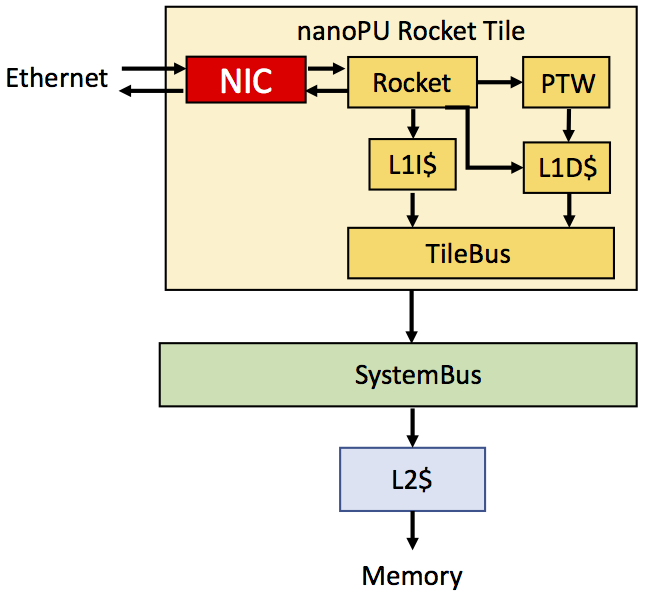
\includegraphics[width=0.75\linewidth]{./figures/nanoPU-prototype}
  \caption{Block diagram of \name{} RISC-V prototype.}
  \label{fig:nanoPU-prototype}
\end{figure}

\begin{figure}
    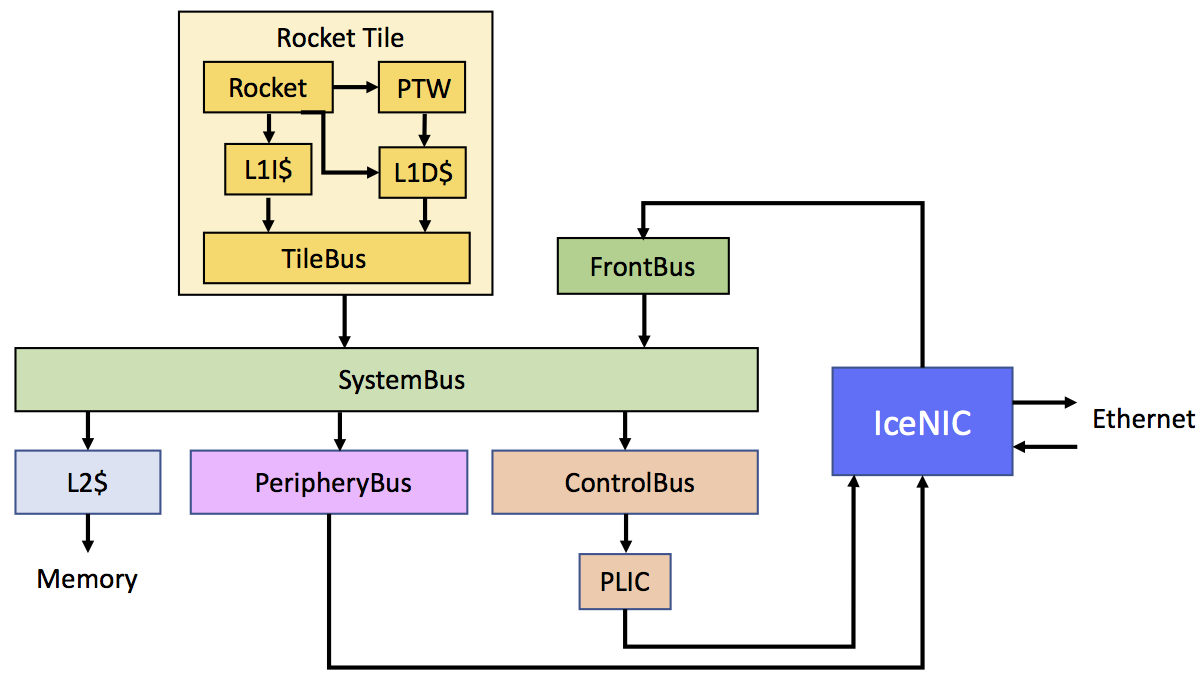
\includegraphics[width=\linewidth]{./figures/icenic-prototype}
    \caption{Block diagram of a traditional RISC-V system with a DMA-based NIC called IceNIC.}
    \label{fig:icenic-prototype}
\end{figure}